\section{Background}

\subsection{The Process Confinement Problem}

The \textit{process confinement problem}, also known as the \textit{sandboxing problem}, refers to the goal of isolating a process or group of processes from the rest of the running system. In practice, this is often achieved by restricting an application's possible behaviour to its desired functionality, explicitly targeting its access to security-sensitive system resources such as files, network interfaces, and other running applications.  Despite decades of work following Lampson's \cite{lampson1973_a_note} first proposal of the process confinement problem in 1973, process confinement remains a somewhat open problem to date \cite{crowell2013_confinement_problem}.

\todo{Discuss OS facilities at a high level, the reference monitor abstraction for access control}

% TODO: Graft parts of the following into threat model in section 3
%\subsection{The Confinement Threat Model}
%\label{subsection:threat_model}
%
%To understand why process confinement is a desirable goal in operating system
%security, we must first identify the credible threats that process confinement
%addresses. To that end, here I describe three attack vectors
%(\crefrange{a:1}{a:3}), followed by three attack goals (\crefrange{g:1}{g:3})
%which highlight just a few of the threats posed by unconfined processes to
%system security, stability, and user privacy.
%
%\begin{enumerate}[label=\bfseries A\arabic*., ref=A\arabic*, labelindent=1em]
%    \item \label{a:1} \textsc{Compromised processes.} Unconfined running
%    processes have classically presented a valuable target for attacker
%    exploitation. With the advent of the Internet, web-facing processes that
%    handle untrusted user input are especially vulnerable, particularly as they
%    often run with heightened privileges \cite{cohen1996_secure}. An attacker
%    may send specially crafted input to the target application, hoping to
%    subvert its control flow integrity via a classic buffer overflow,
%    return-oriented programming \cite{shacham2007_rop}, or some other means. The
%    venerable Morris Worm, regarded as the first computer worm on the Internet,
%    exploited a classic buffer overflow vulnerability in the \texttt{fingerd}
%    service for Unix, as well as a development backdoor left in the
%    \texttt{sendmail} daemon \cite{spafford1989_morris}. In both cases, proper
%    process confinement would have eliminated the threat by preventing
%    the compromised programs from impacting the rest of the system.
%
%    \item \label{a:2} \textsc{Semi-honest software.} Here, I define semi-honest
%    software as that which appears to perform its desired functionality, but
%    which additionally may perform some set of unwanted actions without the
%    user's knowledge. Without putting a proper external confinement mechanism in
%    place to restrict the behaviour of such an application, it may continue to
%    perform the undesired actions \textit{ad infinitum}, so long as it remains
%    installed on the host. As a topical example, an \texttt{strace} of the
%    popular Discord \cite{discord} voice communication client on Linux reveals
%    that it repeatedly scans the process tree and reports a list of \textit{all
%    applications} running on the system, even when the user has turned off the
%    \enquote{display active game} feature\footnote{This feature allows Discord
%    to report, in the user's status message, what game the user is currently
%    playing. The \enquote{display active game} feature appears to be the
%    original motivation behind scanning the process tree.}. This scanning
%    behaviour represents a clear violation of the user's privacy expectations.
%
%    \item \label{a:3} \textsc{Malicious software.} In contrast to semi-honest
%    software, malicious software is that which is expressly designed and
%    distributed with malicious intent. Typically, this software would be
%    downloaded by an unsuspecting user either through social engineering
%    (e.g.~fake antivirus scams) or without the user's knowledge (e.g.~a drive-by
%    download attack). In the case of a computer virus, malicious software may
%    replicate itself on the host by infecting other (originally benign) binaries.
%    It would be useful to provide the user with a means of running such
%    potentially untrustworthy applications in a sandbox so that they cannot
%    damage the rest of the system.
%\end{enumerate}
%
%\begin{enumerate}[label=\bfseries G\arabic*., ref=G\arabic*, labelindent=1em]
%    \item \label{g:1} \textsc{Installation of backdoors/rootkits.} Potentially,
%    the most dangerous attack goal in the exploitation of unconfined processes
%    is the establishment of a backdoor on the target system.  A backdoor needn't
%    be sophisticated---for example, installing the attacker's RSA public key in
%    \texttt{ssh}'s list of authorized keys would be sufficient---however, the
%    most sophisticated backdoors may result in permanent and virtually
%    undetectable escalation of privilege. For instance, a sophisticated attacker
%    with sufficient privileges may load a \textit{rootkit}
%    \cite{beegle2007_rootkit} into the operating system kernel, at which point
%    she has free reign over the system in perpetuity (unless the user manages
%    to somehow remove the rootkit or reinstalls the infected operating system).
%
%    \item \label{g:2} \textsc{Information leakage.} An obvious goal for attacks
%    on unconfined processes (and indeed the focus of the earliest literature on
%    process confinement \cite{lampson1973_a_note}) is information leakage. An
%    adversary may attempt to gain access to personal information or other
%    sensitive data such as private keys, password hashes, or bank credentials.
%    Depending on the type of information, an unauthorized party may not even
%    necessarily require elevated privileges to access it---for instance, no
%    special privileges are required to leak the list of processes running on
%    a Linux system (as in the case of Discord \cite{discord} highlighted above).
%
%    \item \label{g:3} \textsc{Denial of service.} A compromised process could be
%    used to mount a denial of service attack against the host system. For
%    example, an attacker could take down network interfaces, consume system
%    resources, kill important processes, or cause the system to shut down or
%    reboot at an inopportune moment.
%\end{enumerate}
%
%As shown in the examples above, unconfined processes can pose significant
%threats to system security and stability as well as user privacy. The advent of
%the Internet has exacerbated many of these threats. Unconfined network-facing
%daemons continually process untrusted user input, resulting in an easy and
%highly valuable target for attacker exploitation. Email and web browsers have
%enabled powerful social engineering and drive-by download attacks, which often
%result in the installation of malicious software. Semi-honest software can
%violate user expectations of security and privacy by performing unwanted actions
%without the user's knowledge. It is clear that a solution is needed to mitigate
%these threats---for this, we turn to process confinement.

\subsection{Low-Level Isolation Techniques}
\label{subsection:low_level}

The Linux kernel supports various lower-level abstractions for implementing virtualization and enforcing least-privilege. While many of these mechanisms are insufficient for a full confinement implementation on their own, they are typically used in \textit{combination} by higher-level techniques such as containers (c.f.~\Cref{subsection:containers}) to achieve confinement. This section covers these low-level abstractions in detail.

\todo{Go over each of the following subsections, since they are mostly unchanged from the literature review}

\paragraph*{Unix Discretionary Access Control}

Discretionary access control (DAC) forms the most basic access control mechanism in many operating systems, including popular commodity operating systems such as Linux, macOS, and Windows.  First formalized in the 1983 Department of Defense standard \cite{orange_book}, a DAC system partitions system objects (e.g.~files) by their respective owners and allows resource owners to grant access to other users, at their discretion.  Typically, systems implementing discretionary access control also provide an exceptional user or role with the power to override discretionary access controls, such as the superuser (i.e.~\texttt{root}) in Unix-like operating systems and the Administrator role in Windows.

While discretionary access controls themselves are insufficient to implement proper process confinement, they form the basis for the bare minimum level of protection available on many operating systems; therefore, they are an important part of the process confinement discussion. In many cases, user-centric discretionary access controls are abused to create per-application \enquote{users} and \enquote{groups}. For instance, a common pattern in Unix-like systems such as Linux, macOS, FreeBSD, and OpenBSD is to have specific users reserved for security-sensitive applications such as network-facing daemons. The Android mobile operating system takes this one step further, instead assigning an application- or developer-specific UID (user ID) and GID (group ID) to \textit{each} application installed on the device \cite{android_security}.

In theory, these abuses of the DAC model would help mitigate the potential damage that a compromised application can do to the resources that belong to other users and applications on the system. However, due to DAC's discretionary nature, nothing prevents a given user from granting permissions to all other users on the system, unless other measures are put in place. Further, the inclusion of non-human users into a user-centric permission model may result in a disparity between an end-user's expectations and the reality of what a \enquote{user} is. This gap in understanding could result in further usability and security concerns.

\paragraph*{POSIX Capabilities}

Related to discretionary access control are POSIX capabilities \cite{posix_capabilities,corbet2006_capabities_a,corbet2006_capabities_b}, which can be used to grant additional privileges to specific processes, overriding existing discretionary permissions. Further, a privileged process may \textit{drop} specific capabilities that it no longer needs, retaining those it needs. Consequently, POSIX capabilities provide a finer-grained alternative to the all-or-nothing superuser privileges required by certain applications. For instance, a web-facing process that requires access to privileged ports has no business overriding file permissions. POSIX capabilities provide an interface for making such distinctions. Despite these benefits, POSIX capabilities have been criticized for adding additional complexity to an increasingly complex Linux permission model \cite{corbet2006_capabities_b,corbet2006_capabities_a}.  Further, POSIX capabilities do nothing to confine processes beyond the original DAC model---rather, they help to solve the problem of overprivileged processes by limiting the privileges that they require in the first place.

\paragraph*{Namespaces and Cgroups}

In Linux, \textit{namespaces} and \textit{cgroups} (short for control groups) allow for further confinement of processes by restricting the system resources that a process or group of processes is allowed to access. Namespaces isolate access by providing a process group a private, virtualized naming of a class of resources, such as process IDs, filesystem mountpoints, and user IDs. As of version 5.6, Linux supports eight distinct namespaces, depicted in \Cref{tab:namespaces}.  Complementary to namespaces, cgroups limit the use of \textit{quantities} of system resources, such as CPU, memory, and block device I/O.  Namespaces and cgroups provide fine granularity for limiting a process's view of available system resources. In this sense, they are better classified as a mechanism for implementing virtualization rather than least-privilege. They thus must be combined with other measures to constitute a full confinement implementation.

\begin{table}
\begin{tabular}{lp{3in}}
    \toprule
    Namespace & Isolates \\
    \midrule
    \multirow{1}{*}{PID} & Process IDs (PIDs)\\
    \multirow{1}{*}{Mount} & Filesystem mountpoints\\
    \multirow{1}{*}{Network} & Networking stack\\
    \multirow{1}{*}{UTS} & Host and domain names\\
    \multirow{1}{*}{IPC} & Inter-process communication mechanisms\\
    \multirow{1}{*}{User} & User IDs (UIDs) and group IDs (GIDs)\\
    \multirow{1}{*}{Time} & System time\\
    \multirow{1}{*}{Cgroup} & Visibility of cgroup membership\\
    \bottomrule
\end{tabular}
\caption{Linux namespaces (as of kernel version 5.6) and what they can be used to isolate.}
\label{tab:namespaces}
\end{table}

\paragraph*{System Call Interposition}
\todo{This will be adapted from my literature review}

\paragraph*{Linux Security Modules}

The Linux Security Modules (LSM) API \cite{wright2002_lsm} provides an extensible security framework for the Linux kernel, allowing for the implementation of powerful kernelspace security mechanisms that can be chained together. LSM works by integrating a series of strategically placed \textit{security hooks} into kernelspace code. These hooks roughly correspond with boundaries for the modification of kernel objects. Multiple security implementations can hook into these LSM hooks and provide callbacks that generate audit logs and make policy decisions. \Cref{fig:lsm} depicts the LSM architecture in detail.

\begin{figure}[htpb]
    \centering
    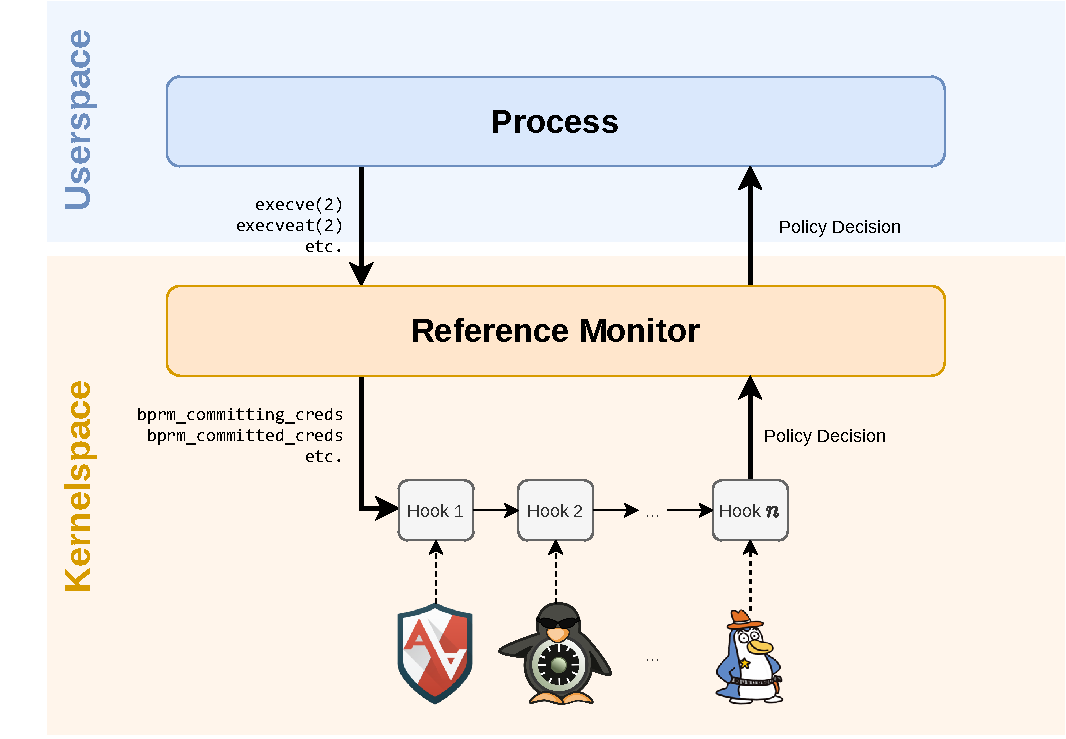
\includegraphics[width=0.8\linewidth]{figs/lsm.pdf}
    \caption{The LSM architecture. Note the many-to-many relation between access
    requests and hook invocations. Multiple LSM hooks may be chained together,
    incorporating policy from many security mechanisms. All hooks must agree to
    allow the access or it will be denied.}%
    \label{fig:lsm}
\end{figure}

The LSM API sits at a level of abstraction just above the system call API---a single LSM hook may cover multiple system calls and a single system call may contain multiple such LSM hooks. For instance, the \texttt{execve(2)} and \texttt{execveat(2)} calls both result in a call to the \texttt{bprm\_committing\_creds} and  \texttt{bprm\_committed\_creds} hooks (among others).  This provides a nice level of abstraction compared to system-call-based approaches like seccomp-bpf \cite{seccomp_bpf, drewry2012_seccomp_bpf} in that a single LSM hook can cover all closely related security events (recall the issue of \texttt{open(2)} vs \texttt{openat(2)} in Seccomp-bpf).

The Linux kernel contains several in-tree LSM-based security modules, which may be enabled by default on certain distributions.  Many such modules implement \textit{mandatory access control} (MAC) schemes, which enable fine-grained access control that can limit the privileges of \textit{all users}---even the superuser. SELinux \cite{smalley2001_selinux} and AppArmor \cite{cowan2000_apparmor} are two such MAC LSMs, each with its own policy semantics. I discuss each in turn.

SELinux \cite{smalley2001_selinux} was originally developed by the NSA as a Linux implementation of the Flask \cite{spencer1999_flask} security model.  Under SELinux, system subjects (users, processes, etc.) and system objects (files, network sockets, etc.) are assigned corresponding labels. Security policy is then written based on these labels, specifying the allowed access patterns between a particular object type and subject type. SELinux's policy language is famously arcane \cite{schreuders12_towards}. Despite multiple efforts to introduce automated policy generation \cite{audit2allow, macmillan07_madison, sniffen06_guided}, writing and auditing SELinux security policy remains a task for security experts rather than end-users. Further, due to the difficulty of writing and auditing the complex SELinux policy language, there is a natural tendency for human policy authors to err on the side of over-permission, violating the principle of least privilege.

AppArmor (originally called SubDomain) \cite{cowan2000_apparmor} is often touted as a more usable alternative to SELinux, although usability studies have shown that this claim merits scrutiny \cite{schreuders12_towards}. Rather than basing security policy on labelling system subjects and objects, AppArmor instead employs path-based enforcement. AppArmor defines policy in per-application profiles, which contain rules specifying what system objects the application can access. System objects are identified directly (for example, via pathnames, socket classes, or IP network addresses) rather than labelled.  AppArmor also supports the notion of \textit{changing hats}, wherein a process may change its AppArmor profile under certain conditions specified in the policy.  Although AppArmor profiles are more conforming to standard Unix semantics than their SELinux counterparts, users who wish to write AppArmor policy still require a considerable amount of knowledge about operating system security \cite{schreuders12_towards}.

\subsection{Containers}
\label{subsection:containers}

Containers use OS-level virtualization and confinement mechanisms (c.f.~\Cref{subsection:low_level}) to provide a (semi-)isolated environment for the execution of processes \cite{sultan2019_container_security}. Since they run directly on the host operating system and share the underlying OS kernel, containers do not require a full guest operating system to implement virtualization. This technique has the advantage of offering a light-weight alternative to traditional hardware virtualization approaches using full virtual machines \cite{sultan2019_container_security}. Compared with containers, traditional approaches to virtualization involve hypervisors, which virtualize and provide access to the underlying hardware, either running on top of a host operating system or directly on top of the hardware itself. Full virtual machines run on top of these hypervisors, each running a guest operating system with a full userland and kernel. Full virtualization provides stronger isolation guarantees than containers but involves significantly more overhead imposed by the guest operating system \cite{sultan2019_container_security}. \Cref{fig:virt} depicts an overview of the architectural differences between containers and full hardware virtualization solutions (i.e.~virtual machines running on top of hypervisors).

\begin{figure}[htpb]
  \centering
  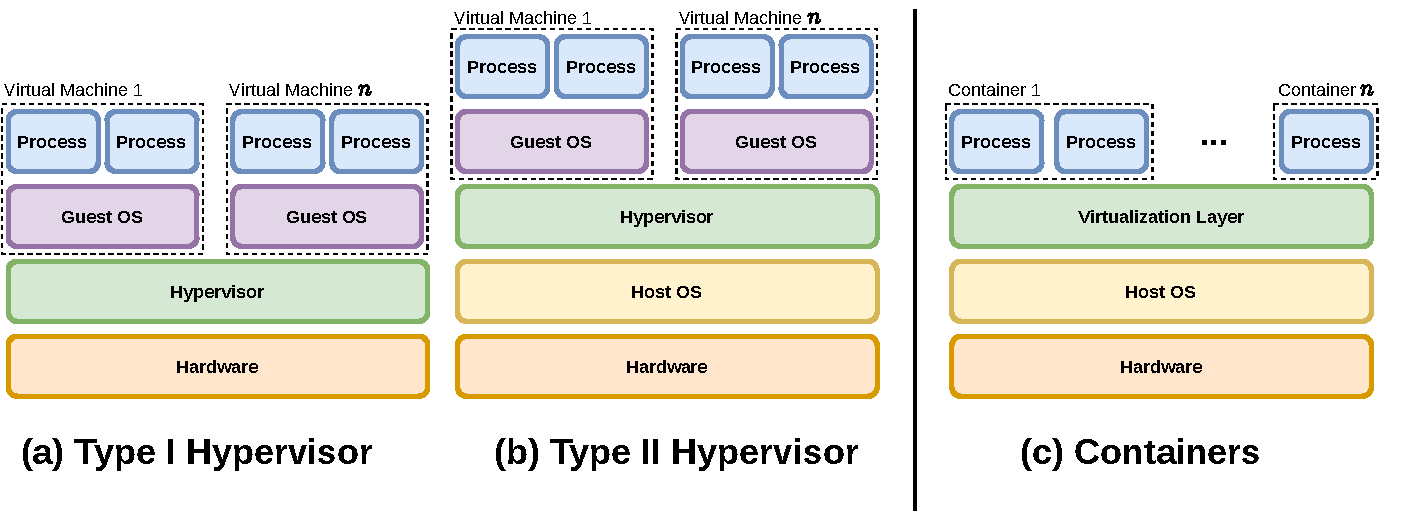
\includegraphics[width=0.8\linewidth]{figs/virtualization.pdf}
  \caption{
    Virtual machine and container architectures. Type I hypervisors \textbf{(a)} virtualize and control the underlying hardware directly, but require full guest operating systems on top of the virtualization layer. Type II hypervisors \textbf{(b)} run on top of a host operating system but still require full guest operating systems above the virtualization layer. Containers \textbf{(c)} achieve virtualization using a thin layer provided by the host operating system itself. They share the underlying operating system kernel and resources, and therefore require no guest operating system \cite{sultan2019_container_security}.
  }%
  \label{fig:virt}
\end{figure}

Since containers must share the host operating system kernel and related resources, it is essential to consider how best to isolate them from one another. Therefore, a container management system generally seeks to achieve the following security-related goals\footnote{Dependency management is another goal of container management systems like Docker \todo{cite}, but it is out of scope for his paper.}:
\begin{enumerate}[label=\bfseries CG\arabic*., ref=CG\arabic*, labelindent=1em]
  \item \textsc{Virtualization.}
    Virtualization aims to provide each container a \textit{virtual view} of system resources. Containers generally achieve virtualization using a combination of Linux namespaces, cgroups, and filesystem mounts. Namespaces provide a private view of enumerable resources (i.e.~a virtual mapping of IDs to resources). Such enumerable resources include process IDs, user and group IDs, mountpoints, and the network interfaces. Cgroups similarly provide a virtual view of \textit{quantifiable resources} (i.e.~how much of a given resource is available). Such quantifiable resources include the CPU, persistent storage, memory, and I/O bandwidth. Filesystem mounts, combined with mount namespaces, provide a virtual view of visible files.

    Although full virtualization may be desirable in the ideal case, containers often only implement partial virtualization \cite{sultan2019_container_security,xin2018_container_security} due to a variety of factors. Pragmatically, it is often beneficial for containers to have a shared view of specific system resources, depending on the use case. For instance, two containers might share a copy of the same shared library or require access to a shared IPC namespace to enable communication. In practice, containers often leverage layered filesystems such as overlayfs \cite{edge2010_overlayfs} to deduplicate files across containers and the host system. Partial virtualization can enable lighter-weight containers and easier communication between two containers to satisfy the goal of composability \cite{sultan2019_container_security}.

  \item \textsc{Least-Privilege.}
    For a container to be considered secure, it must enforce least-privilege on its processes \cite{sultan2019_container_security}. This requirement makes practical sense, given that a container runs directly on the host system and must share the underlying OS kernel and resources with both other containers and the host system itself. Without least-privilege, a process running in a container has virtually the same access rights as an unconfined process. When the container itself is running with privileged access to the system (as is often the case \cite{sultan2019_container_security,xin2018_container_security}), this may even result in an \textit{escalation of privilege} compared to the scenario where the process runs directly on the host. For these reasons, it is neither practical nor advisable to rely on weak virtualization guarantees to protect the host system with no means of enforcing least-privilege \cite{sultan2019_container_security}.

    A least-privilege implementation for containers typically involves a combination of multiple enforcement mechanisms, including Unix DAC, seccomp-based system call filtering, dropped POSIX capabilities, and mandatory access control mechanisms (using one of the Linux MAC LSMs) \cite{sultan2019_container_security,xin2018_container_security,docker}. This complexity can lead to usability and auditability concerns, as a simple policy language must compile down to multiple complex enforcement mechanisms that need to work cooperatively \cite{findlay2020_bpfbox}.

    Despite its evident importance for container security, existing container management solutions generally treat least-privilege as a secondary goal \cite{sultan2019_container_security}. Docker attempts to provide sensible security defaults for containers. Still, these defaults may be easily overridden and often rely on the presence of extra kernel security features such as the AppArmor LSM \cite{docker}. When AppArmor is not available, Docker falls back to relying exclusively on its default seccomp policy and dropped capabilities. Security defaults for containers also often do not adhere to the principle of least privilege. For instance, Docker provides containers with 15 Linux capabilities by default, including \texttt{CAP\_DAC\_OVERRIDE}, which allows a container to override all discretionary access control checks \cite{sultan2019_container_security,docker}.

  \item \label{item:composability} \textsc{Composability.}
    Increasingly, containers are being used to implement composable microservices \cite{sultan2019_container_security}. For instance, Kubernetes \cite{kubernetes} allows the user to group containers into \textit{pods}, which are then allowed to communicate with each other in pre-defined ways. For composability, a container needs to be able to communicate with another container without sacrificing virtualization or least-privilege. In practice, containers achieve such composability by defining specific inter-container exceptions to virtualization and least-privilege policy \cite{sultan2019_container_security}. Naturally, these exceptions can increase the risk of an insecure configuration and the user must carefully manage them to avoid overprivilege.
\end{enumerate}

\todo{Discuss prominent examples: Docker, Kubernetes}

\todo{Discuss containerized package management: Snap, FlatPak}

\subsection{Classic and Extended BPF}

The original Berkeley Packet Filter (BPF) \cite{mccanne1993_bpf}, hereafter referred to as Classic BPF, was a packet filtering mechanism implemented initially for BSD Unix. Classic BPF was created as a lightweight replacement for traditional packet filtering mechanisms, which relied on frequent context switches between userspace and kernelspace while making filtering decisions. Instead, Classic BPF implemented a simple register-based virtual machine language and efficient buffer data structures to minimize the required context switches. As an efficient packet filtering mechanism, Classic BPF quickly gained traction in the *NIX community and was subsequently ported to various open-source Unix and Unix-like operating systems, most notably Linux \cite{linux_bpf}, OpenBSD \cite{openbsd_bpf}, and FreeBSD \cite{freebsd_bpf}.

The Linux kernel development community eventually realized that the BPF engine could be applied to more than just packet filtering. The 2012 introduction of seccomp-bpf \cite{drewry2012_seccomp_bpf,seccomp_bpf} enabled Classic BPF programs to be written and applied to make system call filtering decisions for userspace applications. This extension to seccomp transformed it into a powerful (yet notoriously difficult-to-use \cite{anderson2017_comparison}) mechanism for making security decisions about system calls in a confined process.

In 2014, Starovoitov and Borkmann merged a complete rewrite of the Linux BPF engine, dubbed Extended BPF (eBPF), into the mainline kernel \cite{starovoitov2014_ebpf}. eBPF expands on the original BPF specification by introducing:
\begin{itemize}
  \item An extended instruction set;
  \item 11 registers (10 of which are general-purpose);
  \item Access to allow-listed kernel helpers;
  \item Just-in-time (JIT) compilation to native instruction sets;
  \item A program safety verifier;
  \item A large collection of specialized data structures; and
  \item New program types which can be attached to a variety of system events in both userspace and kernelspace.
\end{itemize}
These extensions to the Classic BPF engine effectively turn eBPF into a general-purpose execution engine in the kernel with powerful system introspection and kernel extension capabilities. eBPF programs execute in the kernel with supervisor privileges but are limited by a restricted execution context and pre-checked for safety by an in-kernel verification engine. In particular, eBPF programs are limited to a 512-byte stack, cannot access unbounded memory regions, must not have back-edges in their control flow, and must provably terminate \cite{gregg2019_bpf}. As a consequence of these restrictions, eBPF programs are not Turing-complete. Where necessary, an eBPF program can make calls to a set of allow-listed kernel helpers to obtain additional functionality, such as access to external memory regions and various kernel facilities such as signalling or random number generation \cite{gregg2019_bpf}.

\begin{figure}[htpb]
  \centering
  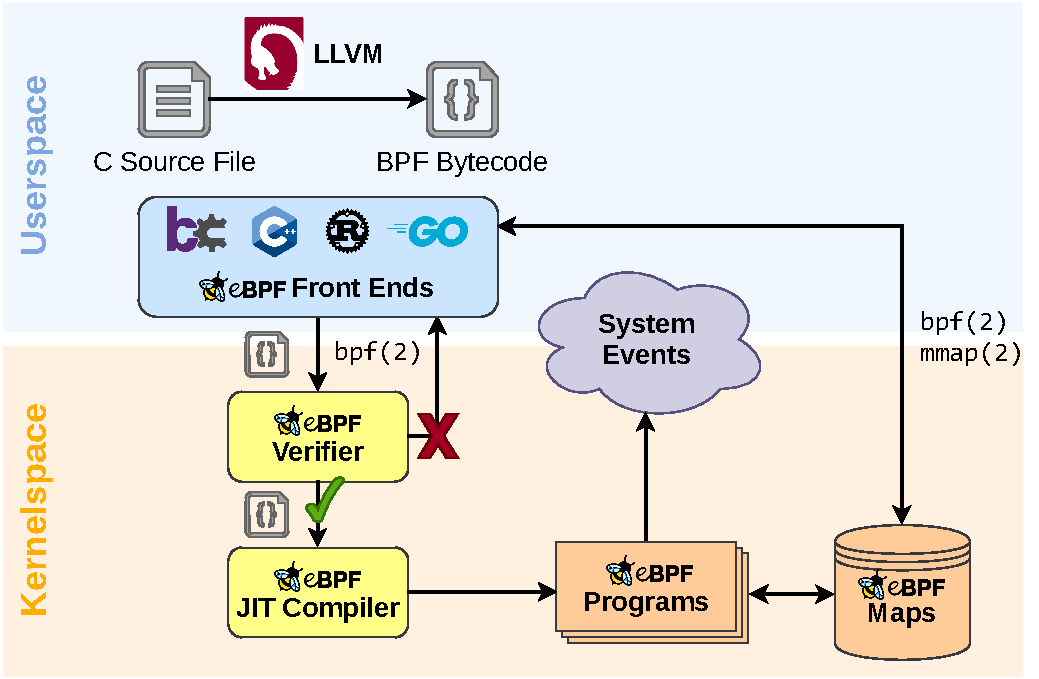
\includegraphics[width=0.8\linewidth]{figs/ebpf.pdf}
  \caption{
    eBPF mechanisms in the kernel. Userspace front-ends compile C source code into eBPF bytecode using the LLVM toolchain and load it into the kernel with the \texttt{bpf(2)} system call. The in-kernel verifier either accepts or rejects the program based on its adherence to safety invariants. Accepted programs are attached to system events across the userspace and kernelspace boundary where they are just-in-time compiled to the native instruction set. Programs can store and fetch data using data structures called \enquote{eBPF maps} which can also be accessed directly from userspace.
  }%
  \label{fig:ebpf}
\end{figure}

A privileged userspace process may load an eBPF program into the kernel using Linux's \texttt{bpf(2)} system call. While it is possible to write eBPF bytecode by hand \cite{gregg2019_bpf}, several front-ends exist for compiling eBPF bytecode from a restricted subset of the C programming language\footnote{In principle, this language need not be C. For instance, a framework exists for writing eBPF programs in pure Rust \cite{redbpf}. However, C is a popular choice since it is tightly coupled with the underlying implementation of the kernel.}, including bcc \cite{bcc} and libbpf \cite{libbpf}. These front-ends typically use the LLVM \cite{llvm_bpf} compiler toolchain to produce BPF bytecode. When the kernel receives a request to load an eBPF program, it first checks the bytecode to ensure that it conforms to the safety invariants outlined above. If the verifier accepts the program, it may then be attached to one or more system events. When an event fires, the eBPF program is executed via just-in-time compilation to the native instruction set. eBPF programs can store data in several specialized in-kernel data structures, which are also made accessible to userspace via the \texttt{bpf(2)} system call or a direct memory mapping. \Cref{fig:ebpf} depicts this process in detail.

